\scanpage{97}
La représentation naturelle de \deleted{$D_{\widetilde P}$}
\[
\tag{6}D_{\widetilde P_{2n}}\overset{\mathrm{def}}=\operatorname{Aut}_{\mathrm{comb}}(\widetilde P_{2n})
\qquad(\simeq D_{2n})
\]
sur $V_{\widetilde P_{2n}}$ définit une action de $D_{\widetilde P_{2n}}$ sur $\boldsymbol\Sigma_{\widetilde P_{2n}}$ et par là sur $\Sigma$, mais qui est triviale sur le sous-groupe $\pm1$, et se factorise donc par une action de
\[
\tag{7}D_{P_n}\overset{\mathrm{def}}=\operatorname{Aut}_{\mathrm{comb}}(P_n)
\simeq D_{\widetilde P_{2n}}/\{\pm1\}
\]
sur $\Sigma=\Sigma_{P_n}$, qui n'est autre que son action naturelle par transport des structures, quand on interprète $\Sigma$ directement comme défini en termes de $P_n$.

\deleted{\unsure{Si}} Si $n$ est impair, la suite exacte canonique

\diagram{\begin{tikzcd}[ampersand replacement=\&]
1\arrow[r,no head]\&\{\pm1\}\arrow[r,no head]\&D_{\widetilde P_{2n}}\arrow[r,no head]\&D_{P_n}\arrow[r,no head]\&1
\end{tikzcd}}
(8)

est scindée \deleted{naturellement} (le \inserted{choix d'un} scindage dépendant du choix d'un \inserted{des deux} ``sous-$n$-gônes'' $P'_n,P''_n$ du $2n$-gône combinatoire $\widetilde P_{2n}$ (pour $n=6$, le choix d'un des deux triangles $ABC$, $A'B'C'$ marqués sur la figure). Cela est lié au fait qu'on a une équivalence de catégories, \uuline{pour $n$ impair}

\figure{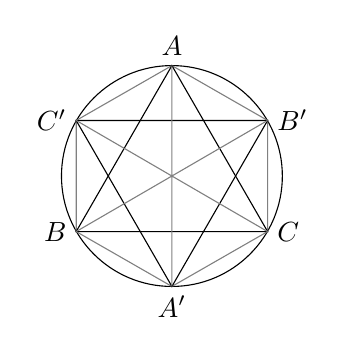
\begin{tikzpicture}[scale=.85]
\coordinate (A) at (0,1.65);
\coordinate (Bp) at (1.43,.83);
\coordinate (C) at (1.43,-.83);
\coordinate (Ap) at (0,-1.65);
\coordinate (B) at (-1.43,-.83);
\coordinate (Cp) at (-1.43,.83);
\draw (0,0) circle (1.65);
\draw[gray] (A)--(Bp)--(C)--(Ap)--(B)--(Cp)--cycle;
\draw (A)--(B)--(C)--cycle;
\draw (Ap)--(Bp)--(Cp)--cycle;
\draw[gray] (A)--(Ap) (B)--(Bp) (C)--(Cp);
\node[above] at (A) {$A$};
\node[right] at (Bp) {$B'$};
\node[right] at (C) {$C$};
\node[below] at (Ap) {$A'$};
\node[left] at (B) {$B$};
\node[left] at (Cp) {$C'$};
\end{tikzpicture}}

\margin{96}
